\pagebreak
\section{Vehicle Tests - Steering - Steering Gain} \label{app:steeringGainTest}
\textbf{Name: Group 510}\\
\textbf{Date: 29/11 - 2015}

\subsection{Purpose}
The purpose of the test is to find the relationship between the vehicle's velocity and its steering. This relationship is described as a steering gain, \si{K_{steering}}.

% find the needed order of the steering model, and the gain related to the speed during the turning of the vehicle, with a PWM signal as an input and the vehicle's heading angle as an output.

\subsection{Theory}
As seen on \secref{sec:SteeringModel}, \figref{basicSteering}, the steering behavior is described with two gain coefficients, \si{K_s} and \si{K_v}. Since their respective value are not needed independently, it is possible to combine them to find a value more easily. The steering gain, \si{K_{steering}}, is therefore defined as :
\begin{flalign}
\eq{K_{steering}}{K_s \cdot K_v}&\nonumber
\end{flalign}
%
Moreover, to get reliable data from which to draw conclusions, a basic proportional controller is implemented to stabilize the angle and realize a step response, as seen on \secref{sec:steeringController}, \figref{fig:basicSteeringWithControl}. 
However, this model is simplified by ignoring the servomotor's delay. Since the test is only a one step response, this delay should only appear once between the step command to the servo and the actual reaching of the desired heading.
Furthermore, since the two summation blocks add a \si{\pm K_{off}}, the offset in the microcontroller cancels the offset from the plant. This way, the model used in this test includes the controller, \si{K_p}, the steering gain, \si{K_{steering}}, and the integrator which allows to get headings out of the vehicle's angular velocity, see \figref{fig:steeringTestWPController}.
%
\begin{figure}[H]
  \centering
  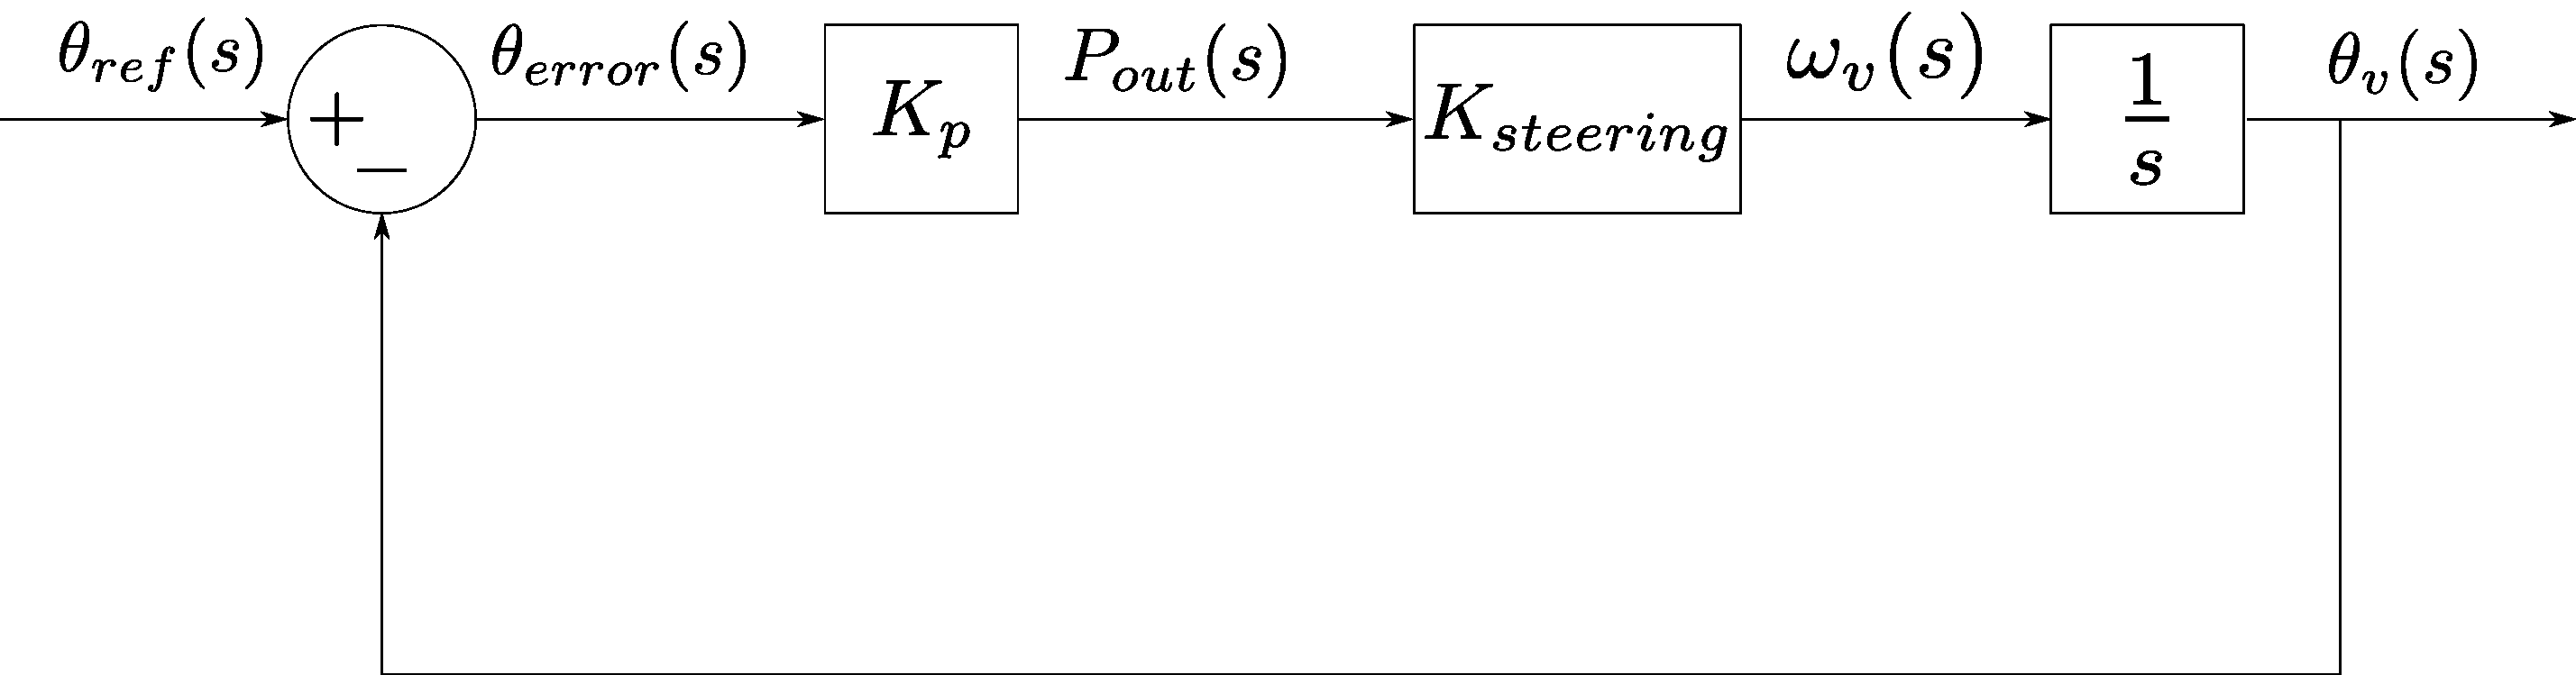
\includegraphics[scale=0.3]{figures/steeringTestWPController.pdf}
  \caption{A diagram of the test setup}
  \label{fig:steeringTestWPController}
\end{figure}

The resulting transfer function of this system can be expressed in standard form as:
\begin{flalign}
\eq{\frac{\theta(s)}{\theta_{ref}(s)}}{\frac{1}{\frac{1}{K_p \cdot K_{steering}}\cdot s + 1}}&
\label{eq:steeringTestWPcontroller}
\end{flalign}

By applying a known reference heading with a fixed gain in the controller and using a steady velocity, the measured parameters are the real heading, real velocity and the timestamp of each measurement point.

\subsection{Setup}
\begin{figure}[H]
  \centering
	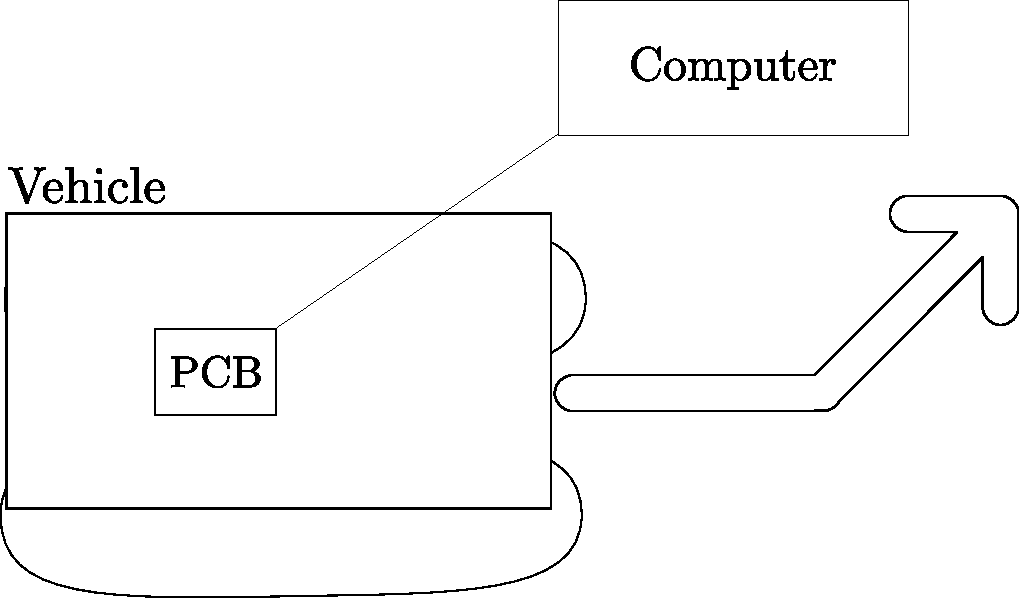
\includegraphics[scale=0.6]{figures/inertiaTestSetupDiagramTurning.pdf}
	\caption{A diagram of the test setup}
\end{figure}

\subsection{List of Equipment}

\begin{table}[H]
\begin{tabular}{|p{10cm}|p{4cm}|}
\hline%------------------------------------------------------------------------------------
  \textbf{Instrument}                     &  \textbf{Type}       \\
\hline%------------------------------------------------------------------------------------
  Computer                                &  Acer C720p    \\
\hline %-----------------------------------------------------------------------------------
\end{tabular}
\end{table}

\subsection{Procedure}

\begin{enumerate}
  \item Make sure the vehicle's power is off.
  \item Connect the Arduino to the computer.
  \item Upload the test code to the Arduino board using the Arduino IDE  \cite{ArduinoIDE}.
  \item Place the vehicle with an orientation of approximately \si{0\ ^{\circ}}, i.e. heading North.
  \item Put the general power on.
  \item Open a serial terminal via PuTTY \cite{PuTTY} immediately after plugging the power in.
  \item Wait two seconds, then follow the vehicle with the connected computer.
  \item Wait until the vehicle stops before ending the measurements by unplugging the connected computer from the Arduino.
  \item Shut the vehicle's power off.
  \item Redo the test multiples while increasing the wanted speed.
  \item Plot the angle of the vehicle using Matlab.
\end{enumerate}

\subsection{Results}
The vehicle is made to run for \si{4000\ ms} with a reference heading of \si{0 ^{\circ}}. The vehicle shall try to head towards the exact magnetic North within these few seconds. After that, the reference angle is put to \si{-45 ^{\circ}} (East) which means the vehicle turns to the right to reach this heading. It goes on running until \si{15\ s} have passed.

From \eqref{eq:steeringTestWPcontroller}, the time constant is found as:
\begin{flalign}
\eq{\tau}{\frac{1}{K_p \cdot K_{steering}}} \unit{s}
\end{flalign}

From this equation and by findig the time constant in each test, it will then be possible to calculate \si{K_{steering}}:
\begin{flalign}
\eq{K_{steering}}{\frac{1}{K_p \cdot \tau}} \unit{rad \cdot s^{-2}}
\label{SteeringTimeconstant}
\end{flalign}
%
The different steering time constants are obtained thanks to the measurement tests. The value of \si{\tau} corresponds to the time when the angle reaches \si{63,2\%} of the final value. A plot of these tests can be seen on \figref{plotStepResponseSteering}. 

\begin{figure}[H]
  \centering
 	%Trim margins @:   left        bottom       right       top
 	\adjustbox{ trim = {.15\width} {.30\height} {.15\width} {.30\height}, clip }
  {
    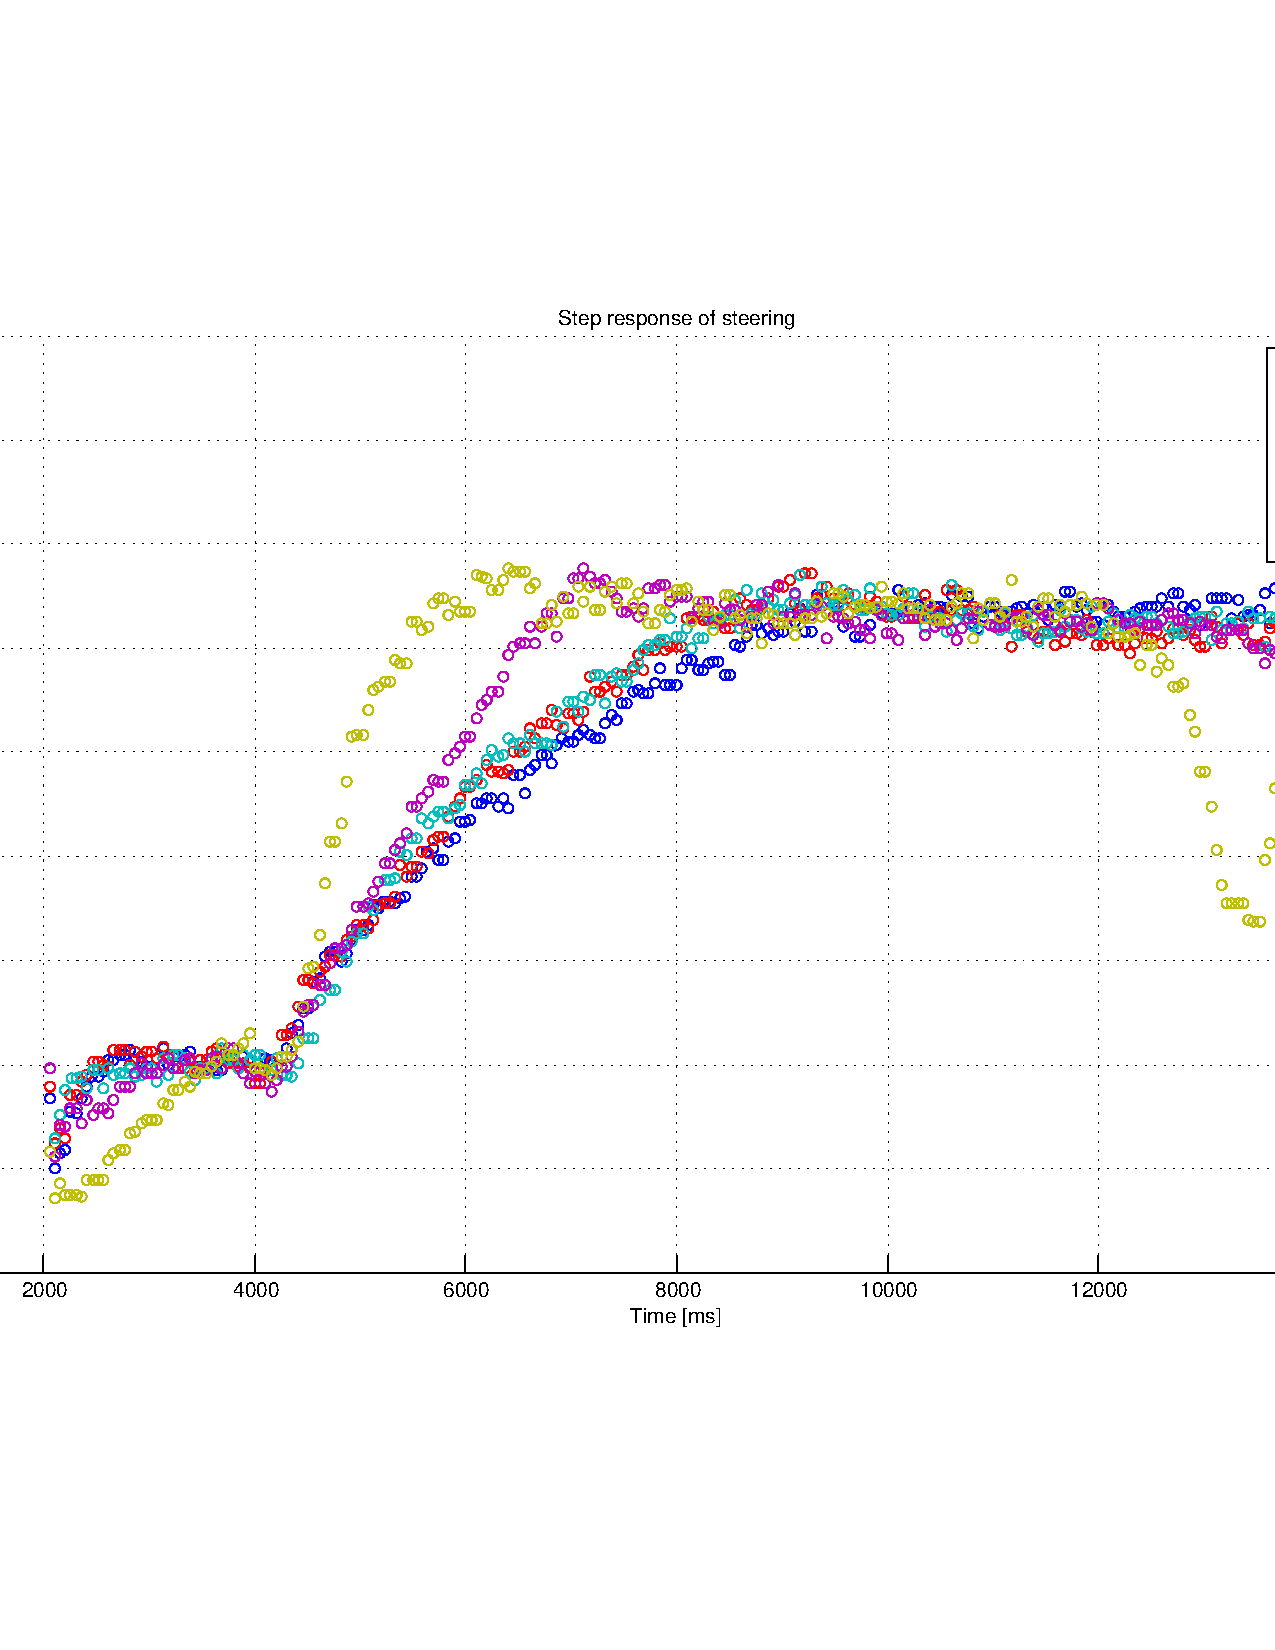
\includegraphics[width=1.4\textwidth]{figures/plotStepResponseSteering.pdf}
  }
  \caption{Plot of multiples step responses for finding the time constant \si{\tau} relative to a specific speed.}
  \label{plotStepResponseSteering}
\end{figure}
%
As the test were made with a choosen control gain \si{K_p = 1,5}, the steering gain is calculated and plotted against the real speed of the vehicle during the turnings, see \figref{steeringPlotSpeedVsGain}.
%
\begin{figure}[H]
  \centering
 	%Trim margins @:   left        bottom       right       top
 	\adjustbox{ trim = {.15\width} {.30\height} {.15\width} {.30\height}, clip }
  {
    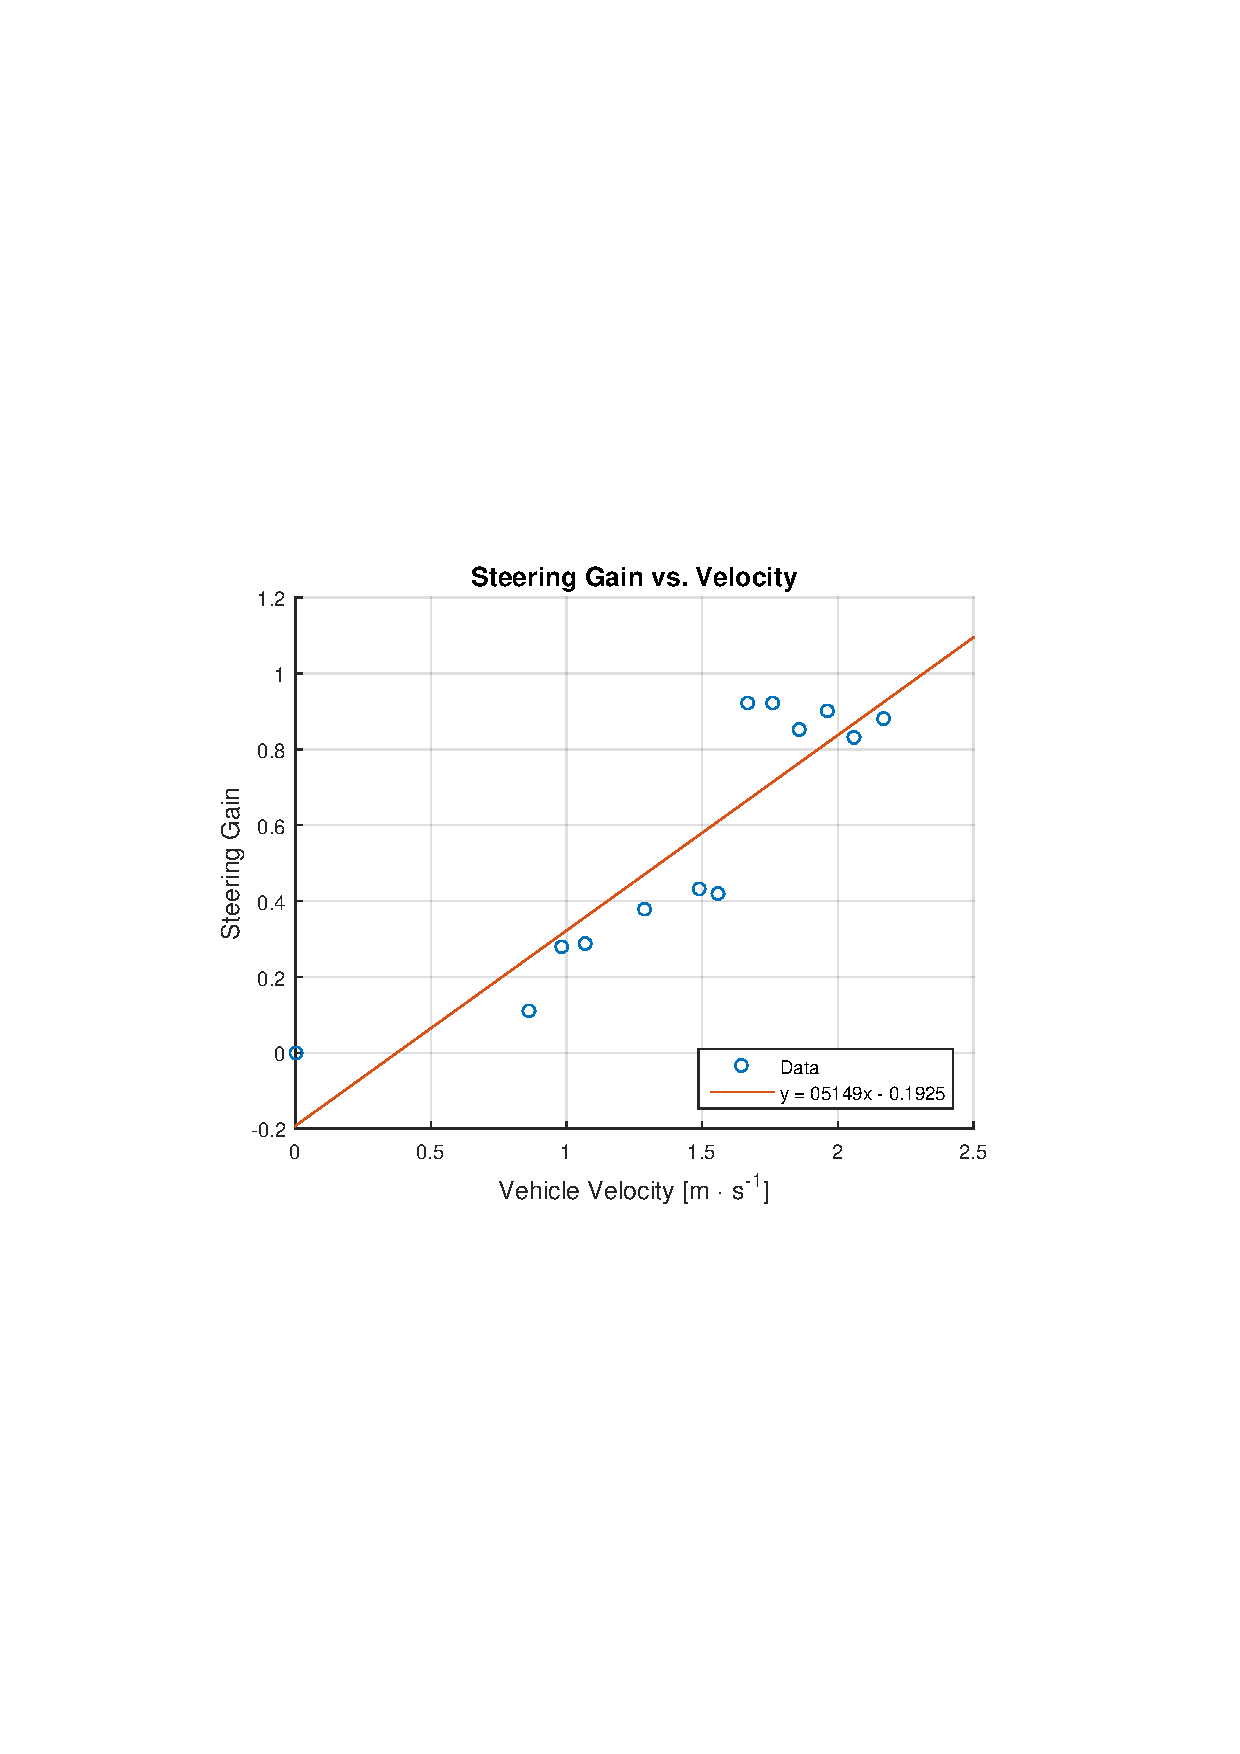
\includegraphics[width=1.4\textwidth]{figures/steeringgainfunction.pdf}
  }
  \caption{Plot of the gain \si{K_v} against the real speed.}
  \label{steeringPlotSpeedVsGain}
\end{figure}
\todo{Fix the axis legend (units)}

From this plot the linear gain proportional to the speed can be established:
\begin{flalign}
\eq{K_{steering}}{0,5149 \cdot v - 0,1925}
\end{flalign}